\section{Methods}\label{sec:methods}

\revised{This section describes the synthetic and real data, how we prepared and explored them, how we
selected variables, and the models and concession extractor we built.}

\subsection{Data}\label{sec:data}

\revised{The original project proposal described a prepared seed dataset covering two to three U.S. metro
markets, roughly 10,000 to 20,000 buildings and 500,000 listing observations, with concession text,
property photos, and analyst-curated comparable sets. In our first meetings, we learned that the
real data was not yet available, so we began with synthetic data. As Accolade advised, we used the
synthetic data to develop and test the pipeline, not to select or tune models. The real Dwellsy
listing data arrived on October~22; we describe it at the end of this subsection.}

The synthetic data was built to conform to the structure of the real data: a market-relative
dataset, which mirrors the Dwellsy listings feed, and a demand pricing dataset, which mirrors a
property's own management-system records. It simulates \nBuildings{} apartment buildings in three
markets, Chicago (\nChicago{}), Dallas--Fort Worth (\nDfw{}), and Washington, DC (\nDc{}), from
\historyStart{} to \asOf{}, across \nSourceTables{} tables and \nSourceRowsM{} million rows. We
organize these tables in three layers (\cref{fig:pipeline}):

\begin{description}[leftmargin=1.5em, labelindent=0pt, font=\normalfont\bfseries]
  \item[Market] what a listings feed observes: buildings, floor plans, every listing with its dated
  price changes, and the free-text specials advertised with them.
  \item[Operator] full property-management records for \nPms{} buildings, including leases, guest
  cards, and a reference system's daily price recommendations, which we will use in Phase~2.
  \item[Truth] the values the generator drew before anything was observed, such as each floor plan's
  true market rent by month, each listing's true lease, and each building's latent quality and
  pricing policy.
\end{description}

\revised{The truth layer makes the synthetic data especially useful.} A real listings feed only
records what landlords asked, whereas this data also records what each unit was worth, so we can
evaluate whether a method recovers the market rent rather than whether it simply reproduces the
listings.

By default, the generator describes an unremarkable, stabilized building with 12-month leases, fully
priced and with nothing missing, and it then enables named edge cases on top. Attributes are masked:
\yearBuiltMasked{} of buildings are missing a year built and \storiesMasked{} a story count.
\nLeaseUp{} buildings are delivered partway through the history and lease up from empty,
\rmShare{} of buildings reprice daily under revenue management while the rest adjust by hand,
\nVacancySpikes{} vacancy spikes disrupt individual buildings, and \nRentControlled{} buildings in DC
are rent-controlled. Concessions appear in \nConcessionEvents{} advertised specials written in
varied prose. Because each edge case is named, the generator can double as a test harness for the
data-quality problems we expect in the real data.

One caution applies throughout. Because the generator builds rent from building attributes, a
flexible model can score well partly by recovering the generator's own formula. Therefore, we treat
our synthetic results as evidence that a method works when the data behaves as assumed, not as a
forecast of its accuracy on real listings.

\revised{The real data is a trial extract from Dwellsy, the listing provider. It covers \dwListings{}
listings of \dwUnits{} rental units in the Chicago and Washington, DC metropolitan areas between
\dwStart{} and \dwEnd{}, with the same 47 variables in both markets. We analyze Chicago first:
545,312 listings of 152,233 units, so a unit appears 3.6 times on average. The target is
\texttt{rent\_amount}, the advertised monthly rent, which is never missing. The main predictors are
the unit's bedrooms, bathrooms, and square footage, the building's year built and property type, its
ZIP code and coordinates, and the listing date. Most are nearly complete, but year built is 32\%
missing and half bathrooms 83\% missing. Unlike the synthetic data, the real data has no truth
layer, so we can score models only against asking rent.}

\subsection{Preprocessing}\label{sec:preprocessing}

\revised{We first merged} the \nMasterTables{} source tables relevant to rent prediction into a
master table with one row per listing, \nMasterRows{} listings by \nMasterCols{} columns. Building
and floor-plan attributes join one-to-many, while a listing's price history and advertised specials
are aggregated to the listing. Every join is checked for duplicated rows, and every column keeps the
name of its source table (for example, \texttt{market\_building\_\_year\_built}), so its origin stays
clear after any selection. \revised{We then reviewed each variable's content and
standardized its data type as a string, float, integer, date, or boolean.}

A column's name, however, does not tell us whether it can be used. We therefore also tagged each
column with a role (feature, label, latent, or leaky) and \revised{selected} inputs by role under a single rule:
an input must be known on the day the unit is listed. \Cref{fig:leakage} shows why this rule has to
be enforced by role rather than by correlation. Nine columns are the listing's own later prices and
correlate with asking rent at \(|r| \geq \minLeakyLevelR\), so they are easy to catch. Four more are
the same prices per square foot, with \(|r| \approx \psfAloneR\), no higher than the best legitimate
variable, so a correlation screen would keep them. Yet multiplied by square footage, they reproduce
asking rent to within 1\% for \psfExactShare{} of \nPsfRows{} listings (\(r = \psfTimesSqftR\)). A
model given these columns would score almost perfectly and learn nothing~\autocite{kaufman2012leakage}.

\begin{figure}[htbp]
  \centering
  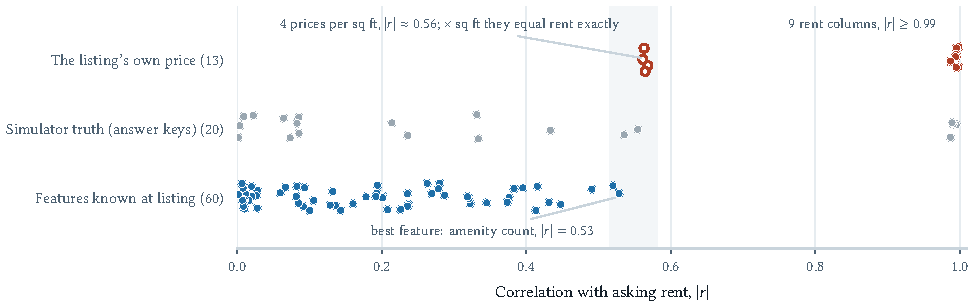
\includegraphics{leakage}
  \caption{Correlation of every numerical column with asking rent, by role. Variables known when a
  unit is listed (blue) reach \(|r| = \maxFeatureR\). The listing's own later prices (red) are
  leaks: nine rent columns are obvious, but four prices per square foot (open circles) fall in the
  shaded band beside the best variable, where correlation cannot tell them apart. Grey points are the
  generator's answer keys, never used as inputs.}
  \label{fig:leakage}
\end{figure}

\revised{For the real Chicago listings, our checks for invalid values found only one, a listing with a
non-positive square footage, so we kept every listing. We dropped half bathrooms and impute the
remaining missing values inside the modeling pipeline, fitted on the training set only: medians for
numerical variables and the most frequent value for categorical ones. Because units are listed
repeatedly, we split the data by rental unit into training (64\%), validation (16\%), and test
(20\%) sets. No unit appears in more than one set, so a model cannot score well by memorizing units
it has already seen.}

\subsection{Exploratory data analysis}\label{sec:eda}

Our exploratory analysis of the synthetic data focused on how rent varies across markets, unit types, and buildings, and on
which variables carry information about it. Median asking rent is \medRentDc{} in DC,
\medRentChicago{} in Chicago, and \medRentDfw{} in Dallas--Fort Worth (\cref{fig:map}). Between
\firstYear{} and \lastYear{} it rose by \growthChicago{} in Chicago and \growthDc{} in DC, while in
Dallas--Fort Worth it peaked in \dfwPeakYear{} and has since leveled off. Within each market, rent
generally rises with the number of bedrooms, but the spread within each bedroom count is wide
(\cref{fig:ladder} \revised{in \cref{app:figures}}), which suggests that location and building characteristics matter as much as the
size of the unit.

Unit size shows why the building level matters. Across all listings, square footage has a Pearson
correlation of \sqftOverallR{} with asking rent, but within a single building the correlation rises
to \sqftWithinR{}. In other words, size explains rent much better once the building is held fixed,
because buildings also differ in many other ways that affect price. \revised{Some promising variables,
however, are mostly missing:} \nSparseFees{} fee and parking variables have
Spearman correlations between \sparseRhoLo{} and \sparseRhoHi{} with rent, but are \sparseMissLo{} to
\sparseMissHi{} missing.

\revised{The real Chicago listings show the same building effect, though weaker: square footage
correlates with asking rent at 0.51 across all listings and 0.65 within a community, so comparable
selection should help on real data too. Two differences from the synthetic data matter for
modeling. Median asking rent in Chicago stayed between about \$1,500 and \$1,830 per quarter from
2021 to 2026, far flatter than the synthetic data's \growthChicago{} rise, so synthetic trends
should not guide real-data choices. The number of listings per quarter also fell from about 50,000
in 2021 to about 15,000 in 2025 and 2026, so most training data comes from the earliest years, and
we will also test on the most recent period.}

\begin{figure}[htbp]
  \centering
  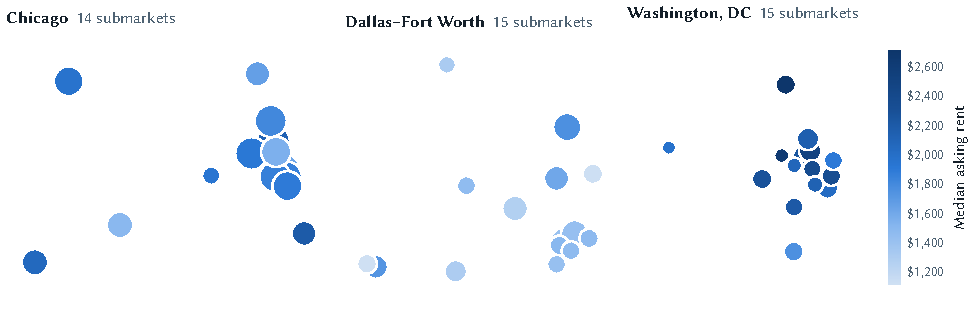
\includegraphics{rent_map}
  \caption{Median asking rent by submarket. Each circle is one submarket, sized by its number of
  listings and colored on one scale across the three markets.}
  \label{fig:map}
\end{figure}

\subsection{Feature selection}\label{sec:selection}

To narrow the \nMasterCols{} columns down to the model's inputs, we followed a staged funnel
(\cref{fig:funnel}, in \cref{app:figures}). After removing keys, answer keys, and leaky columns, \nFeatureCols{} columns
remain, of which \nKnownCols{} are known when a unit is listed. We then analyzed the numerical and
categorical variables separately.

For the numerical variables, we used two complementary approaches. The first scored every numerical
variable with Gini, gradient boosting importance, and Lasso, and kept \nKeptNumeric{} of the
\nNumCandidates{} candidates. The second applied univariate, bivariate, and multivariate stages in
sequence, narrowing 65 numerical predictors to 44 and then 18. The two selections agree on ten core
variables, led by unit size (Spearman correlation of \sqftSpearman{} with rent) together with
location, the building's amenity count and review score, its leasing exposure when the unit was
listed, and three measures of how often the building changes its prices.

\revised{For the categorical variables, we first profiled the 215 boolean and 28 categorical predictors
against the target. We found that cardinality has to be judged per building rather than per row.} A street address is only 0.31\% distinct across listings but 99.97\% distinct across
buildings, so it is effectively a building identifier rather than a category. We therefore excluded
identifiers and chose which categorical variables to keep based on their importance on buildings the
model had not seen. Six of the \nCatCandidates{} candidates are kept: property class, ZIP code, floor
plan name, unit name, the predicted story bucket, and management company. On their own, they reach
an \(R^2\) of 0.55 on held-out buildings.


\subsection{Models}\label{sec:models}

Our initial models, developed using synthetic data, predict the first asking rent of a listing, 
the price posted when the unit comes on the market. As inputs we use \nFeatures{} numerical 
variables known at that point: unit size, bedrooms,
bathrooms, and floor; the building's amenities, review score, size, age, and application fee; its
location; and the number of units sharing the floor plan. We compared three models: linear
regression as an interpretable reference, a decision tree for its readable splits, and gradient
boosting~\autocite{friedman2001greedy} to capture nonlinear relationships. Missing values are imputed
with the median for linear regression and the decision tree, while gradient boosting, implemented as
scikit-learn's histogram-based gradient boosting~\autocite{ke2017lightgbm, pedregosa2011scikit},
handles them natively. As a reference point, we also include a naive baseline that predicts the
median rent for the listing's market and bedroom count. \Cref{app:models} lists the settings.

\revised{On the real Chicago listings, we compared five regression models: linear regression, a decision
tree, a random forest, histogram-based gradient boosting, and a baseline that predicts the mean
training rent. They use eight predictors: bedrooms, full bathrooms, square footage, year built, ZIP
code, property type, and the listing's year and month, with ZIP code and property type one-hot
encoded. We compare the models on the validation set and keep the test set for the final model. To
test whether exact location adds information beyond ZIP code, we also fit a Ridge regression with
spline transformations of latitude and longitude.}

\subsection{Concession extraction}\label{sec:concession-methods}

As a first step toward Phase~2, we built a rule-based extractor for concession terms. Advertised
specials are free text, such as ``Enjoy the first month free on a 13-month lease,'' and Phase~2 needs
their value in dollars to compute effective rent. We found that the concession type is already
recorded in the market data and agrees with the truth layer for every one of the
\nConcessionEvents{} specials, so only the value has to be extracted from the text. The extractor
reads the amount, its basis (months free or dollars), and the lease term, and we score it against
the truth layer.
